\documentclass[floatfix,nofootinbib,superscriptaddress,fleqn]{revtex4-2}  
%\documentclass[aps,epsfig,tightlines,fleqn]{revtex4}
\usepackage[utf]{kotex}
\usepackage[HWP]{dhucs-interword}
\usepackage[dvips]{color}
\usepackage{graphicx}
\usepackage{bm}
%\usepackage{fancyhdr}
%\usepackage{dcolumn}
\usepackage{defcolor}
\usepackage{amsmath}
\usepackage{amsfonts}
\usepackage{amssymb}
\usepackage{amscd}
\usepackage{amsthm}
\usepackage[utf8]{inputenc}
 \usepackage{setspace}
 \usepackage{tikz}
 \usetikzlibrary{decorations,decorations.markings,decorations.text}
%\pagestyle{fancy}

\begin{document}
\pgfkeys{/pgf/decoration/.cd,
distance/.initial=10pt
}  

\pgfdeclaredecoration{add dim}{final}{
\state{final}{% 
\pgfmathsetmacro{\dist}{5pt*\pgfkeysvalueof{/pgf/decoration/distance}/abs(\pgfkeysvalueof{/pgf/decoration/distance})} 
          \pgfpathmoveto{\pgfpoint{0pt}{0pt}}             
          \pgfpathlineto{\pgfpoint{0pt}{2*\dist}}   
          \pgfpathmoveto{\pgfpoint{\pgfdecoratedpathlength}{0pt}} 
          \pgfpathlineto{\pgfpoint{(\pgfdecoratedpathlength}{2*\dist}}
           \pgfusepath{stroke} 
          \pgfsetdash{{0.1cm}{0.1cm}{0.1cm}{0.1cm}}{0cm}     
          \pgfsetarrowsstart{latex}
          \pgfsetarrowsend{latex}  
          \pgfpathmoveto{\pgfpoint{0pt}{\dist}}
          \pgfpathlineto{\pgfpoint{\pgfdecoratedpathlength}{\dist}} 
          \pgfusepath{stroke} 
          \pgfsetdash{}{0pt}
          \pgfpathmoveto{\pgfpoint{0pt}{0pt}}
          \pgfpathlineto{\pgfpoint{\pgfdecoratedpathlength}{0pt}}
}}

\tikzset{dim/.style args={#1,#2}{decoration={add dim,distance=#2},
                decorate,
                postaction={decorate,decoration={text along path,
                                                 raise=#2,
                                                 text align={align=center},
                                                 text={#1}}}}}


\title{\Large 2022년 1학기 물리학 I: Quiz 16}
\author{김현철\footnote{Office: 5S-436D (면담시간 매주
    화요일-16:00$\sim$20:00)}} 
\email{hchkim@inha.ac.kr}
\affiliation{Hadron Theory Group, Department of Physics,
Inha University, Incheon 22212, Republic of Korea }
\date{Spring semester, 2022}


\vspace{1.cm}

\maketitle


\noindent {\bf 문제 1. (40 pt)}
높이가 5 m인 큰 수족관에 2.00 m의
깊이로 민물이 채워져 있다. 폭이 8.00 m인 수족관의 한쪽 벽은 두꺼운
플라스틱으로 만들어져 있다. 물을 더 채워 수심이 4.00 m가 되었다면,
벽에 가해지는 전체 힘은 얼마나 증가하겠는가? 

\noindent {\bf 풀이 : }
벽이 받는 전체 힘 $F$, 민물에 의한 압력 $P$, 민물과 벽이 닿는 면적 $A$
\begin{align}
  F = \int P\,dA,\,\,\,P = \rho g h
\end{align}
폭 $a$, 민물의 높이 $h$, 미소면적 $dA$
\begin{align}
  dA = a\,dh
\end{align}
처음 높이 $h_1$, 처음 힘 $F_1$
\begin{align}
  F_1 = \int_0^{h_1}\rho g h\,dh = \frac{1}{2}\rho g h^2_1
\end{align}
나중 높이 $h_2$, 나중 힘 $F_2$
\begin{align}
  F_2 = \int_0^{h_2}\rho g h\,dh = \frac{1}{2}\rho g h^2_2
\end{align}
힘의 변화량 $\Delta F$,
\begin{align}
  \Delta F = F_2 - F_1 = \frac{1}{2}\rho g \left(h^2_2-h^2_1\right)
\end{align}
% 대기압 $P_0$, 수면으로부터 깊이 $h$ 인 곳에서의 압력 $P_h$ 
% \begin{align}
%   P_h = \rho g h +P_0.
% \end{align}
% 벽이 받는 미소 압력 $dP$
% \begin{align}
%   dP = \rho g \,dh
% \end{align}
% 벽이 받는 전체 압력 $P$
% \begin{align}
%   P = \int^h_0 \rho g \,dh^\prime
% \end{align}
% 처음 깊이 $h_1$, 처음 압력 $P_1$,
% \begin{align}
%   P_1 = \int^{h_1}_0\rho g \,dh^\prime
% \end{align}
% 폭을 $a$라 하면 물과 벽이 닿는 면적 $A_1$
% \begin{align}
%   A_1 = h_1a.
% \end{align}
% 벽이 받는 전체 힘 $F_1$
% \begin{align}
%   F_1 = P_1 A_1 =h_1a\left(\int^{h_1}_0\rho g \,dh^\prime \right)
% \end{align}
% 나중 깊이 $h_2$, 나중 압력 $P_2$,
% \begin{align}
%   P_2 = \int^{h_2}_0\rho g \,dh^\prime 
% \end{align}
% 물과 벽이 닿는 면적 $A_2$
% \begin{align}
%   A_2 = h_2a.
% \end{align}
% 벽이 받는 전체 힘 $F_2$
% \begin{align}
%   F_2 = P_2 A_2=h_2a\left(\int^{h_2}_0\rho g \,dh^\prime \right)
% \end{align}
% 힘의 변화량 $\Delta F$,
% \begin{align}
%   \Delta F = F_2 - F_1
%   = h_2a\left(\int^{h_2}_0\rho g \,dh^\prime \right)
%   -h_1a\left(\int^{h_1}_0\rho g \,dh^\prime \right)
%   =a\rho g (h_2^2-h_1^2)
% \end{align}
\vspace{1.cm}


\noindent {\bf 문제 2. (100 pt) {\color{red} 난이도 상}:}
그림~\ref{fig:1}에서처럼 폭이 $W=314$
m인 댐의 상류 쪽에 깊이 $S=35.0$ m만큼 물이 차 있다. 
\begin{figure}[htp]
  \centering
  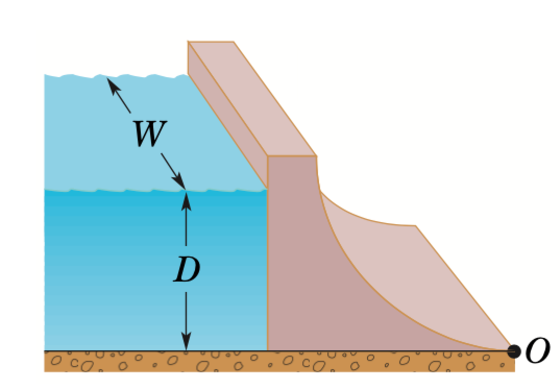
\includegraphics[scale=0.65]{Qfig16-1.pdf}
    \caption{문제 2}
  \label{fig:1}
\end{figure}
\begin{itemize}
\item[(가)] 물의 계기압력(gauge pressure of the water)으로부터 댐에
  가해지는 알짜힘을 구하라.
\item[(나)] 그 힘에 의해 생기는 알짜 돌림힘을 점 $O$를 지나고 댐의
  폭에 형행인 축에 대해 구하여라.
\item[(다)] 돌림힘의 모멘트팔을 구하여라.   
\end{itemize}

\noindent {\bf 풀이 : }
\begin{itemize}
  \item[(가)]
  깊이 $h$에서 물의 계기압력 $P_{\mathrm{gauge}}$는,
  \begin{align}
    P_{\mathrm{gauge}} = \rho g h
  \end{align}
  물과 댐이 닿는 면적 $A$, 계기압력에 의해 댐에 가해지는 힘 $F_{gauge}$는,
  \begin{align}
    F_{\mathrm{gauge}} = \int P_{\mathrm{gauge}}\,dA
  \end{align}
  폭을 $W$라 하면
  \begin{align}
    A = Wh,\,\,\, dA = Wdh
  \end{align}
  힘 $F_{gauge}$는,
  \begin{align}
    F_{\mathrm{gauge}} = \int^S_0 P_{\mathrm{gauge}}\,dA
    =\int^S_0 \rho g W h\,dh = \frac{1}{2}\rho g Wh^2
  \end{align}
  \item[(나)] 물에 닿는 면적에 대해 힘이 연속적으로 작용하므로 
  각 높이에 작용하는 미소힘에 의한 미소돌림힘 $d\tau$를 찾으면
  \begin{align}
    d\tau = r\sin\theta dF,\,\,\,dF=\rho g Wh\,dh
  \end{align}

  \begin{figure}[htbp]
    \begin{tikzpicture}
    \centering
    \coordinate (O) at (4,0);
    \coordinate (A) at (0,0);
    \coordinate (A') at (-1,0);
    \coordinate (S') at (-1,3);
    \coordinate (h) at (0,2);
    \coordinate (h') at (-1,2);
    \coordinate (S) at (0,3);
    \draw[fill] (O) circle (2pt) node [right,black] {$O$};
    \draw[dim={$l$,-15pt}]  (A) --  (O); 
    \draw[dim={$r$, 15pt}]  (h) --  (O);
    \draw[]  (S) -- (A);
    \draw[densely dotted]  (S) -- (S');
    \draw[densely dotted]  (h) -- (h');
    \draw[dim={$S$,-15pt}]  (S) -- (A);
    \draw[dim={$h$, 10pt}]  (h') --  (S');
    \draw[] (3.5,0) arc(180:166:1) 
    (3,0) node[above] {$\theta$};
    \draw[red,very thick,-latex] (h)-- +(1,0)
    node [above,black] {$dF$};
    \end{tikzpicture}
  \end{figure}

  $r\sin\theta=S-h$ 이므로 
  \begin{align}
    d\tau = r\sin\theta dF
    =\rho g W (S-h)h \,dh
  \end{align}
  따라서 총 돌림힘은
  \begin{align}
    \tau =\int_0^S \rho g W (S-h)h \,dh 
    = \rho g W\left(\frac{1}{2}S^3-\frac{1}{3}S^3\right)
    =\frac{1}{6}\rho g WS^3
  \end{align}
  \item[(다)] 모멘트팔의 길이를 $l$이라고 하면
  \begin{align}
    \tau = lF,\,\,\,l = \frac{\tau}{F}
  \end{align}
\end{itemize}

\vspace{1.cm}


\noindent {\bf 문제 3. (60pt)}
그림~\ref{fig:2}처럼 용수철 상수가 $3.00\times 10^4$ N/m인 용수철이
단단한 들보와 유압지렛대의 출력 피스톤 사이에 연결되어 있다.
\begin{figure}[htp]
  \centering
  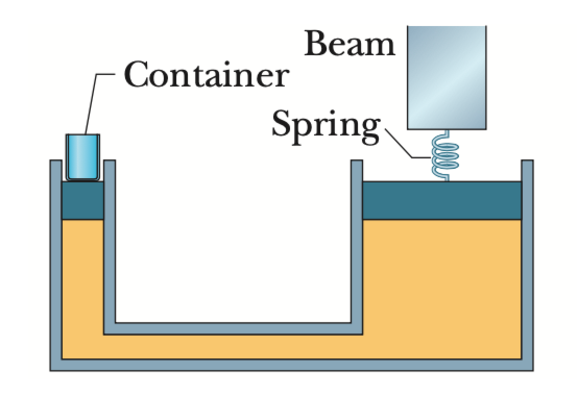
\includegraphics[scale=0.65]{Qfig16-2.pdf}
    \caption{문제 3}
  \label{fig:2}
\end{figure}
 질량을 무시할 수 있는 빈 통이 입력 피스톤 위에 놓여 있다. 입력 피스톤의
단면적은 $A_i$이고 출력 피스톤의 단면적은 $18.0 A_i$이다. 처음에
용수철은 늘어나지 않은 길이이다. 천천히 빈 통에 모래를 부어서 몇 kg을
넣어야 용수철이 $5.00$ cm만큼 수축하겠는가? 

\noindent {\bf 풀이 : }
모래를 $m$만큼 넣었을 때 입력 피스톤에 작용하는 압력 $P_{in}$
 \begin{align}
   P_{in} =\frac{F}{A} =\frac{mg}{A_i}
 \end{align}
 유체가 출력 피스톤에 작용하는 압력 $P_{out}$, 출력 피스톤이 올라가 스프링을 압축시키면 
 스프링은 출력 피스톤에 복원력 $F_{out}$을 가한다. 출력 피스톤이 스프링을 압축시키는 힘과
 스프링의 복원력이 평형을 이루면 출력 피스톤과 스프링은 정지한다. 
 이 때 $P_{out}$과 $F_{out}$는 다음 관계에 있다.
 \begin{align}
   P_{out} = \frac{F_{out}}{18A_i}
 \end{align}
 또한 스프링에 의한 복원력 $F_{out}$은
 \begin{align}
   F_{out} = kx = kh_2,
 \end{align}
 이고 압력 $P_{out}$은
 \begin{align}
  P_{out} = \frac{kh_2}{18A_i}
 \end{align}
 이다. 압력은 유체의 어디에서나 같으므로 $P_{in}=P_{out}$이다. 따라서,
 \begin{align}
  \frac{mg}{A_i} = \frac{kh_2}{18A_i},\,\,\,m=\frac{kh_2}{18g}
 \end{align}
 우리가 구하고자 하는 것은 $h_2 = 5.00\,\mathrm{cm}$일 때 모래의 질량 $m$이므로
\vspace{1.cm}


\noindent {\bf 문제 4. (40pt)}
속이 비어있는 쇠공이 물에 거의 잠긴
채 떠 있다. 바깥 반지름이 60.0 cm이고, 쇠의 밀도가
$7.87\,\mathrm{g/cm^3}$일 때 안쪽 반지름을 구하여라.

\noindent {\bf 풀이 : }
쇠공은 자신이 물속에서 차지한 부피를 가진 물의 무게를 부력으로 받는다.
쇠공이고 물에 거의 잠겨있으므로 바깥쪽 반지름을 $b$라고 하면 
부력 $F_b$는
\begin{align}
  F_b = \frac{4}{3}\pi b^3\rho_0 g
\end{align}
안쪽 반지름 $a$,  밀도 $\rho$, 쇠공이 받는 중력 $F_g$는
\begin{align}
  F_g = mg = \frac{4}{3}\pi(b^3-a^3)\rho g
\end{align}
쇠공은 정지해있으므로 두 힘이 같아 평형을 이룬다. 즉, $F_b = F_g$이고
\begin{align}
  \frac{4}{3}\pi b^3\rho_0 g = \frac{4}{3}\pi(b^3-a^3)\rho g
\end{align}
이다. 안쪽 반지름을 구하기 위해 $a$에 대해 정리하면 다음과 같다.
\begin{align}
  a^3 = \left(1-\frac{\rho_0}{\rho}\right)b^3,\,\,\,
  a = \sqrt[3]{1-\frac{\rho_0}{\rho}}b
\end{align}
수치를 대입해서 구해보면 다음과 같다.
\end{document}